% -*- latex -*-
%-----------------------------------------------------------------------
%;  Copyright (C) 2009
%;  Associated Universities, Inc. Washington DC, USA.
%;
%;  This program is free software; you can redistribute it and/or
%;  modify it under the terms of the GNU General Public License as
%;  published by the Free Software Foundation; either version 2 of
%;  the License, or (at your option) any later version.
%;
%;  This program is distributed in the hope that it will be useful,
%;  but WITHOUT ANY WARRANTY; without even the implied warranty of
%;  MERCHANTABILITY or FITNESS FOR A PARTICULAR PURPOSE.  See the
%;  GNU General Public License for more details.
%;
%;  You should have received a copy of the GNU General Public
%;  License along with this program; if not, write to the Free
%;  Software Foundation, Inc., 675 Massachusetts Ave, Cambridge,
%;  MA 02139, USA.
%;
%;  Correspondence concerning AIPS should be addressed as follows:
%;          Internet email: aipsmail@nrao.edu.
%;          Postal address: AIPS Project Office
%;                          National Radio Astronomy Observatory
%;                          520 Edgemont Road
%;                          Charlottesville, VA 22903-2475 USA
%-----------------------------------------------------------------------
%Body of final AIPSletter for 31 December 2009

\documentclass[twoside]{article}
\usepackage{graphics}

\newcommand{\AIPRELEASE}{December 31, 2009}
\newcommand{\AIPVOLUME}{Volume XXIX}
\newcommand{\AIPNUMBER}{Number 2}
\newcommand{\RELEASENAME}{{\tt 31DEC09}}
\newcommand{\OLDNAME}{{\tt 31DEC08}}
\newcommand{\NEWNAME}{{\tt 31DEC10}}

%macros and title page format for the \AIPS\ letter.
\input LET98.MAC

\newcommand{\MYSpace}{-11pt}

\normalstyle

\section{General developments in \AIPS}

\subsection{Current and future releases}

We have formal \AIPS\ releases on an annual basis.  We recommend a
full binary installation method for both the frozen and development
versions for MacIntosh OS/X (PPC and Intel chips), Solaris, and Linux
(32- and 64-bit) systems, but all architectures can do a full
installation from the source files.  If you develop \AIPS\ code
locally, you will need to do a source-level installation.  The current
release is called \RELEASENAME\ and is now ``frozen.''  If you took a
development copy of this version at some earlier date, you should use
the ``Midnight Job'' (MNJ) to bring it up to date.  You need to run a
MNJ only once in 2010 to convert your copy of \RELEASENAME\ into the
frozen version.  When patches to \RELEASENAME\ are announced, you may
apply them with the MNJ\@.  This \Aipsletter\ is intended to advise
you of corrections and improvements in this release.

We have begun a new version, called \NEWNAME, which is now under
development by the \AIPS\ Group.  You may fetch and install a complete
copy of this version at any time.  Having fetched \NEWNAME, you may
update your installation whenever you want by running the MNJ\@.  This
uses cvs, rsync, and/or transaction files to copy and compile the code
selectively based on the code changes and compilations we have done.
We expect users to take their source-only or binary version of
\NEWNAME\ \AIPS\ over the Internet (via \emph{anonymous} ftp).  Both
versions require you to copy the installation procedure {\tt
install.pl} via {\tt ftp}; the source-only version also requires you
to ftp the 97-Mbyte {\tt \NEWNAME.tar.gz} compressed tar file.  Linux
sites will almost certainly have {\tt cvs} installed; other sites may
have installed it along with other GNU tools.  Secondary MNJs will
still be possible using {\tt ssh} or {\tt rcp} or NFS as with previous
releases.  We have found that {\tt cvs} works very well, although it
has one quirk.  If a site modifies a file locally but in an
\AIPS-standard directory, {\tt cvs} will detect the modification and
attempt to reconcile the local version with the NRAO-supplied version.
This usually produces a file that will not compile or run as intended.

\AIPS\ is now copyright \copyright\ 1995 through 2009 by Associated
Universities, Inc., NRAO's parent corporation, but may be made freely
available under the terms of the Free Software Foundation's General
Public License (GPL)\@.  This means that User Agreements are no longer
required, that \AIPS\ may be obtained via anonymous ftp without
contacting NRAO, and that the software may be redistributed (and/or
modified), under certain conditions.  The full text of the GPL can be
found in the \texttt{15JUL95} \Aipsletter\ and is included with every
distribution in file {\tt \$AIPS\_ROOT/{\it release-name}/COPYING}\@.
\vfill\eject

\subsection{Installing a new version}

If compiling locally, new releases must be installed from the tar ball
for that release.  If using the binary installation, a full new
installation must also be done with {\tt rsync}.  The {\tt cvs} system
requires this.  When installing a new \AIPS\ release in a system that
already has a previous release, we recommend that {\tt install.pl} be
used and that the previous release be left in place, at least until
the new installation has been seen to work.  If you do this, then you
will not have to re-edit the disk, printer, and tape lists and can
simply skip all those pages in the {\tt install.pl} menus.  The old
{\tt \$HOME/.AIPSRC} file may be left in place, but it will need to be
edited.  The lines giving the {\tt DOWNLOADED} and {\tt UNPACKED}
parameters should be cleared and the {\tt CCOMOPT} line should be
changed to point to the current release rather than the previous one
--- the {\tt -I} parameter really should be {\tt -I\$INC} but it gets
its full path name instead.  This forces a re-edit with each release.
If you have made special versions of {\tt UPDCONFIG} and {\tt
do\_daily.{\it host}}, you should preserve them under new names and
restore them after the install.  If you have an odd set of \AIPS\
versions, the {\tt \$AIPS\_ROOT/AIPSPATH.*SH} files may need to be
edited after the install to set the desired versions.

For Linux, Solaris Ultra, and MacIntosh systems, a binary installation
could be available from DVD, supported by {\tt install.pl}.
Alternatively, the frozen version may be installed with the binary
installation method now present in {\tt install.pl}.  The ftp site for
downloading files directly has been eliminated.

\section{\AIPS\ Distribution}

From the NRAO system logs, we count apparent MNJ accesses, downloads
of the tar balls, and {\tt rsync} accesses by unique IP address.
Since DSL and some university and other connections may be assigned
different IP addresses at different times, this will be a bit of an
over-estimate of actual sites.  However, a single IP address is often
used to provide \AIPS\ to a number of computers, so these numbers are
at the same time an under-estimate of the number of computers running
current versions of \AIPS\@.  In 2009, a total of 307 different IP
addresses downloaded the frozen form of \OLDNAME\ and 1228 IP
addresses downloaded \RELEASENAME\ in tarball or binary form.  Fully
1855 IP addresses accessed the NRAO cvs master.  Each of these has at
least installed some version of \AIPS\ and 507 appear to have run the
MNJ at least occasionally.  The total number of unique IP addresses in
these three lists was 2399.  478 sites accessed \OLDNAME\ in binary
form, while 1082 sites used the binary form of \RELEASENAME\@.  The
attached figure shows the cumulative number of unique sites, cvs
access sites, tar-ball/binary download sites and binary access sites
known to us as a function of week in 2009.  These numbers represent
substantial increases (more than 10\%) over those for 2008.

\centerline{\resizebox{4.8in}{!}{\includegraphics{FIG/PLOTIT9b.PS}}}

\vfill\eject

Since the registration system, always under-utilized, has now been
abandoned, we are left with analysis by IP address.  The table below
lists the IP addresses for 2009 by the final qualifier for shipments
of \RELEASENAME, \OLDNAME, and access to the cvs site.  The numbers in
the cvs column include those sites that install or run a midnight job
for these releases.  The comments come from what appears to be a
semi-official list of Internet codes.  Sorting is on the ``unique''
column, which counts unique IP addresses over the other three columns:

\vspace{10pt}
\begin{center}
\begin{tabular}{lrrrrl}
\hline\hline
Code  & {\tt 31DEC08} & {\tt 31DEC09} & cvs site & unique & Comments \\
\hline

net     &   22 &  130 &  490 &  554 &  Network \\
edu     &   34 &  213 &  344 &  401 &  US Educational \\
uk      &   12 &  102 &   85 &  132 &  United Kingdom \\
jp      &   16 &   73 &   50 &   87 &  Japan \\
com     &   15 &   43 &   51 &   74 &  US Commercial \\
de      &    5 &   29 &   61 &   73 &  Germany \\
org     &    6 &   30 &   50 &   57 &  Non-Profit Organization \\
in      &   16 &   29 &   38 &   56 &  India \\
es      &    9 &   33 &   36 &   50 &  Spain \\
pl      &    1 &   32 &   29 &   42 &  Poland \\
it      &    2 &   28 &   25 &   34 &  Italy \\
br      &   20 &   13 &   16 &   30 &  Brazil \\
nl      &    3 &   20 &   25 &   29 &  Netherlands \\
au      &    2 &   12 &   22 &   28 &  Australia \\
ca      &    5 &   15 &   24 &   26 &  Canada \\
fr      &    3 &   21 &   16 &   23 &  France \\
ru      &    2 &   21 &   13 &   22 &  Russian Federation \\
za      &    3 &   10 &    7 &   19 &  South Africa \\
mx      &    4 &   12 &    6 &   14 &  Mexico \\
gov     &    1 &    9 &    6 &   12 &  US Government \\
se      &    0 &    4 &   10 &   10 &  Sweden \\
ie      &    4 &    6 &    6 &    8 &  Ireland \\
mil     &    2 &    2 &    6 &    7 &  US Military \\
tw      &    0 &    6 &    6 &    7 &  Taiwan \\
ar      &    4 &    3 &    3 &    6 &  Argentina \\
fi      &    1 &    4 &    5 &    6 &  Finland \\
be      &    3 &    2 &    3 &    5 &  Belgium \\
cl      &    1 &    3 &    4 &    5 &  Chile \\
pt      &    1 &    1 &    4 &    4 &  Portugal \\
dk      &    1 &    0 &    2 &    3 &  Denmark \\
arpa    &    0 &    3 &    2 &    3 &  Old style Arpanet \\
at      &    0 &    2 &    3 &    3 &  Austria \\
yu      &    0 &    3 &    2 &    3 &  Yugoslavia \\
hu      &    0 &    3 &    1 &    3 &  Hungary \\
nz      &    1 &    1 &    1 &    2 &  New Zealand (Aotearoa) \\
ae      &    1 &    2 &    0 &    2 &  United Arab Emirates \\
lv      &    1 &    2 &    1 &    2 &  Latvia \\
ch      &    1 &    1 &    2 &    2 &  Switzerland \\
gr      &    0 &    2 &    1 &    2 &  Greece \\
cn      &    0 &    2 &    0 &    2 &  China \\
kr      &    1 &    1 &    1 &    1 &  Korea (South) \\
il      &    0 &    1 &    1 &    1 &  Israel \\
bg      &    0 &    1 &    1 &    1 &  Bulgaria \\
sa      &    0 &    1 &    0 &    1 &  Saudi Arabia \\
ro      &    0 &    0 &    1 &    1 &  Romania \\
tr      &    0 &    0 &    1 &    1 &  Turkey \\
%None    &    1 &    8 &   20 &   24 &   \\
%Unknown &  103 &  289 &  374 &  521 &   \\
Unknown &  104 &  297 &  394 &  545 &   \\
\hline
Total   &  307 & 1228 & 1855 & 2399 &   \\
\hline
\end{tabular}
\end{center}

\vfill\eject

\section{Preview of coming attractions}

The \NEWNAME\ release already contains a few changes that we decided
were a bit risky or not needed in \RELEASENAME\@.  {\tt UVRFI} is a
new task that implements two methods for excising RFI from data
without flagging the data samples.  It shows some real promise in
cases which are suited to the algorithm.  The old task {\tt RM} has
already been revised to read image cubes with FQID axes (as now
produced by {\tt FQUBE} and {\tt MCUBE}) and to have an additional
method for searching for the best fit rotation measures.  New tasks
are being developed to evaluate tables and $uv$/image data left behind
by pipelines.  The installation procedure has been given code to avoid
common problems when the site name or architecture changes at a site
installing a new version of \AIPS\@.

\section{Improvements of interest to users in \RELEASENAME}

We expect to continue publishing the \Aipsletter\ every six months
along with the annual releases.  There are a number of new tasks
released in the last 6 months along with a variety of improvements to
{\tt IMAGR} and other tasks.  The new tasks include {\tt FQUBE} to
build image cubes with an {\tt FQID} axis to describe irregularly
distributed frequencies, {\tt FARS} to determine best estimates of
rotation measure by the Faraday rotation synthesis algorithm, {\tt
  CAPLT} to plot closure amplitudes with source models, {\tt SNCOP} to
average IFs within an {\tt SN} table and copy the averages to an {\tt
  SN} table of another data set, {\tt BLCHN} to perform
channel-dependent baseline corrections, {\tt ATLOD} to translate ATNF
and ATLBA data into \AIPS, and {\tt SUFIX} to correct source
assignments in $uv$ data sets.  The new verb {\tt FILEZAP} allows one
to delete an external file from within {\tt AIPS}\@.  {\tt IMAGR} now
can do baseline-length dependent time averaging on input, can switch
from {\tt OVERLAP 2} mode to {\tt OVERLAP 1} mode automatically, and
can delete boxes which overlap in more than one facet.  In the first
half of 2009, {\tt IMAGR} learned how to create Clean boxes
automatically supported by new tasks {\tt SABOX} and {\tt FILIT}\@.
The latter task was improved in recent months as well.

Normally, bugs which are created in an \AIPS\ {\tt TST} version and
then fixed in that same version before its release get little or no
discussion in the \Aipsletter\@.  Since a rather large number of sites
now install the {\tt TST} version of \AIPS\ during its development,
this is somewhat of an oversight.  We urge you to run the ``Midnight
Job'' at least once after \RELEASENAME\ is frozen to bring it up to
date and to fix all bugs of this sort.  We will discuss below a
particular set of errors that accompanied the change in antenna file
format and have set up a web page {\tt
  http://www.aips.nrao.edu/problems.shtml} which we hope to maintain
to emphasize such matters.  It is linked from the main \AIPS\ web page
so it is not necessary to remember the above URL\@.   Other bugs of
this sort are mentioned below for {\tt IMAGR}, {\tt FILIT}, and {\tt
  EDITR}\@.  We urge active sites to use the MNJ and, when something
odd occurs, to examine {\tt CHANGE.DOC} using the cgi tool available
from the \AIPS\ web page under documentation.  Please do not hesitate
to e-mail {\tt daip@nrao.edu} with any questions or suspicions that
there are problems.

\RELEASENAME\ contains a change in the format of antenna files which
will be discussed in detail below.  Previous releases will not
understand the antenna coordinates for arrays that were traditionally
left-handed (VLBI primarily).  The format change occurs automatically
when any \RELEASENAME\ antenna-file specific code reads the file,
after which older releases will have difficulties.  Major changes were
made to the display software last year in \OLDNAME.  Older versions
may use the \OLDNAME\ display ({\tt XAS}), but \OLDNAME\ code may not
use older versions of {\tt XAS}\@.  FITS-IDI data from the DiFX
correlator, now in use for the VLBA, requires {\tt 31DEC08} or later.
{\tt  31DEC04} through \NEWNAME\ use a new numbering scheme for
magnetic tape logical unit numbers that is incompatible with previous
versions.  Thus all tape tasks and the server {\tt TPMON} must be from
a recent release.  Other than these issues, \OLDNAME\ is compatible in
all major ways with the with the {\tt 15OCT98} and later releases.
There are significant incompatibilities with older versions.  Note
that the only version which we patch for major errors is \RELEASENAME;
even \OLDNAME\ is no longer changed.

%\vfill\eject

\subsection{Imaging}

\subsubsection{FARS}

{\tt FARS} is a new task to perform Faraday rotation synthesis on
images of Q and U made at a variety of frequencies.   The user
prepares two cubes of these images using {\tt FQUBE} and {\tt
  TRANS}\@.  The task determines the Faraday rotation free ($\lambda
=0$) brightness and the Faraday depth of the media on the way from the
source to the observer.  The main ideas of the algorithm are described
by M. A. Brentjens and A. G. de Bruyn in Astronomy \&\ Astrophysics,
441, 1217-1228 (2005).  The task Fourier transforms the data at each
spatial pixel along the $\lambda^2$ axis.  A simple version of Hogbom
Clean is used to find a small number (usually 1 or 2) of complex
components.  The position of these components on the transformed axis
corresponds to the rotation measure of that component while the real
and imaginary values correspond to the Q and U of the component.  The
task then produces images of Q, U, and rotation measure for each of
the allowed components.  This task is new and experimental and will
undoubtedly require improvements in the algorithm, in user controls,
and in documentation.  Nonetheless, it offers a significant step up
from the rather simple algorithms in, for example, \AIPS\ task {\tt
  RM}\@.

\subsubsection{IMAGR}

{\tt IMAGR} has acquired yet more capabilities.  Perhaps of greatest
interest, is the new capability to average a time-sorted input file in
time with an averaging interval that depends upon projected baseline
length.  The input parameters are the size of the overall image and
the maximum allowed averaging interval, with the default to do no
averaging.  This should make the task run faster since it can reduce
the size of the work file considerably. It will, however, change the
image some since it will have preferentially averaged short spacing
data, thereby changing the cell sampling seen in uniform weighting.  A
modest taper could be used to compensate.

In high-dynamic range imaging with multiple facets, it is recommended
to begin in {\tt OVERLAP = 2 ; ONEBEAM FALSE} mode for the most
accurate beam pattern and to avoid sidelobes of the strongest sources.
However, when the dynamic range of the residual images is reduced, the
need for this accuracy is very much less.  At that stage, Cleaning all
the facets in each round, perhaps with only one beam, would be rather
faster and of sufficient accuracy.  The new adverb {\tt OVRSWTCH} has
been added to {\tt IMAGR} to have the task itself perform this switch
at an appropriate moment.  This puts the task in {\tt OVERLAP=1} mode
in which overlapping Clean boxes cause instabilities.  Therefore, a
new routine was added to check for overlapping Clean boxes and to drop
the smaller one in each overlap when in this mode.  In {\tt OVERLAP=2}
mode, this clean-up operation is not automatic but is available from
the TV menu.

Another new user option is one that controls whether the Clean of the
next spectral channel starts with all the boxes used for the previous
spectral channel or starts over with whatever boxes were specified in
the inputs and input {\tt BOXFILE}\@.

A number of internal matters were also improved.  {\tt IMAGR} will now
append keywords for average zenith and parallactic angle only for
observations that cover a small time range for which these averages
are then meaningful.  The auto-boxing routine would refuse to make
boxes around single bright pixels, so the routine that finds the
maximum in the residual changed to use the average of adjacent pixels
in pairs for the maximum.  Infinite loops may have been seen by users
until this was fixed.  The Clean Components are now restored to all
resolutions in multi-resolution Clean.  This allows the output images
to be used in {\tt FILIT} and {\tt SABOX} for all resolutions.  {\tt
  OVERLAP = 1} mode seemed to have trouble stopping at a {\tt FLUX}
cutoff.  It would Clean all facets below {\tt FLUX} and then re-image
them finding several very slightly above {\tt FLUX} and so on and so
forth.  The test for ``is there anything to Clean now'' was changed to
use {\tt 1.05 * FLUX} to avoid this useless extra computation.

{\tt IMAGR} is now very much more careful about using a pre-existing
work file.  It did not seem able to confirm that such a file was
actually appropriate for the current input adverbs and so would use
ones that did not have the new parameters.  Pre-existing workfiles are
now deleted unless {\tt ALLOKAY = 2}, which tells the task that the
contents of the workfile are current and useful.  The tests on the
data to determine if sorting to $uv$-plane order had errors which
caused {\tt IMAGR} to sort data rather often when the data did not
need to be sorted.  These are corrected and avoid a potentially lengthy
sort operation.  The code that found a list of model facets which
could be subtracted at the same time had an error that caused the list
making to stop at any facet with no components.  All components were
eventually subtracted, but the data were read more times than
necessary.
\vfill\eject

\subsubsection{Miscellaneous}

\begin{description}
\myitem{FQUBE} is a new task to build image cubes with an irregular
        frequency ID (``{\tt FQID}'') axis for which the correct
        frequencies of each plane are determined by a table look up.
        It is meant to simplify the serious complexities of {\tt
          MCUBE}\@.  {\tt MCUBE} was corrected for a bug limiting the
        output axis to 2048.
\myitem{FILIT} was corrected for bad errors when {\tt OBOXFILE} was
        the same as {\tt BOXFILE}.  It has new options to check boxes
        for overlap between facets, to enter the next facet number
        directly (rather than jumping by $\pm 1$), and to delete all
        boxes in the current facet.
\myitem{IMAGE} extensions in FITS are a standard form which \AIPS\ has
        not previously recognized.  {\tt IMLOD} and {\tt FITLD} were
        changed to recognize this form of FITS file and to make one or
        more images in the \AIPS\ catalog from them.
\myitem{COMB} was changed to copy attached tables other than Clean
        Components.  This enables the {\tt FQ} table to be preserved.
\myitem{SAD} and {\tt IMFIT} and {\tt JMFIT} did incorrect things with
        the image rotation on the deconvolved component parameters
        when one or both widths were indeterminate.
\end{description}

\subsection{UV data}

\subsubsection{Antenna tables}

The format of the \AIPS\ antenna tables was changed.  The main purpose
of the change was to take control of the geometry of the antenna
locations quoted in the file.  Previously, \AIPS\ and other packages
had to know whether right-handed or left-handed geometries were used
according to the array name in the file --- and that was sometimes
uncertain.  Now there are two new header keywords {\tt TFRAME} to
define the terrestrial frame for the antenna locations ({\it e.g.,}
{\tt ITRF}) and {\tt XYZHAND} to define the handedness (now always
{\tt RIGHT}).  An automatic translation occurs using the array or
station names to determine what handedness is used and to force it to
right-handed.  Two columns were added to the antenna file itself, {\tt
  DIAMETER} of the antenna in meters and {\tt BEAMFWHM} of the antenna
as a function of IF in degrees per meter wavelength.  At present these
columns are little used, but there are several heterogeneous arrays
(such as CARMA and ALMA) which have come into operation or soon will
be in use.

This change was introduced into {\tt 31DEC09} en masse on September
20, 2009.  This change will produce errors when the new antenna files
are used by software that does not understand the new handedness, such
as {\tt 31DEC08} and earlier versions of \AIPS\ and other software
packages.  These errors will not produce messages in most cases.  When
{\tt 31DEC09} (or later) touches an antenna file it fixes its format
if needed.  But then, when an older version reads a ``fixed'' VLBI
file it will make a wrong assumption about handedness.  This includes
{\tt UVFIX}, plot routines doing elevation or parallactic angle, {\tt
  CLCOR 'POLR', 'PANG', 'ANTP', 'IONS', 'ATMO'}, {\it  et
  al.\/}~corrections, {\tt UVFLG} elevation flagging, {\tt CALIB}
elevation cutoff for gain normalization, {\tt TECOR}, {\tt ANTAB} with
opacity corrections, {\tt DELZN}, {\tt CAL}, {\tt LPCAL}, {\tt CVEL},
and probably others.  Negative elevations are a common symptom of this
error; use {\tt UVPLT} to plot the elevations in your data to test for
the problem.  A {\tt RUN} file named {\tt ANFIX8} was patched into
{\tt 31DEC08} to correct ``fixed'' antenna files.  Note that VLBA data
pre-processed into the NRAO archive will have the new convention,
causing old \AIPS\ versions to have trouble with the latest archive
data.  Archive files in FITS-IDI format are safe, but more numerous
and bothersome.

Unfortunately, the change also contained a number of outright errors.
{\tt FITLD} was left able to record some antennas with the wrong $B_y$
coordinate if they did not occur in the first FITS-IDI file.  A large
number of archive files affected by this bug are being corrected, but
a procedure {\tt ANCHECK} is available as a {\tt RUN} file to check
your VLBA pre-processed data for this error.

The application of polarization calibration was completely broken in
{\tt 31DEC09} from September 20 to November 17.  The results of {\tt
  PCAL} and friends were probably fine, but the application of those D
terms was badly messed up.  The {\tt POLR} option in {\tt CLCOR}
corrected the {\tt CL} table properly but only corrected the first IF
in the polarization solutions in the antenna table.  That error was
fixed November 26.

The executive summary of the above is that you should use {\tt 31DEC09}
or {\tt 31DEC10} and make sure that your version is up to date.

\subsubsection{Other changes}
\begin{description}
\myitem{CLCOR} was changed so that {\tt 'ANTP'} and {\tt 'ANTC'}
        operations compute delays internally with respect to antenna
        one.  The absolute delays for the EVLA which uses
        Earth-centered antenna coordinates were way too large for
        storage in single-precision.  Note that the {\tt CL} table is
        in single precision which limits the accuracy of large shifts
        for VLBI and other long baselines.
\myitem{FRING} was changed to handle time intervals with only one
        sample and, similarly, to force a delay-only form of solution
        if requested.  The output frequency increment and reference
        pixel were corrected.
\myitem{CALIB} was changed to use {\tt ICHANSEL} rather than {\tt
        BCHAN} and {\tt ECHAN} to define the spectral channels to be
        averaged.
\myitem{BPASS} had an egregious error causing it to average all
        channels rather than use {\tt ICHANSEL} correctly in those
        modes that use that adverb.
\myitem{BLCAL} was changed to use {\tt ICHANSEL}; previously it
        averaged all channels.
\myitem{BLCHN} is an experimental, channel-dependent version of {\tt
        BLCAL}\@.  It produces a {\tt BD} table but applies its
        corrections directly to an output file.  The {\tt BD} table
        can be displayed by {\tt POSSM} and {\tt BPLOT}\@.
\myitem{TVFLG} was corrected for a memory error which caused it to die
        when more than six spectral channels were used.  {\tt TVFLG}
        and {\tt SPFLG} now offer an option of TV transfer functions
        which will be useful for high dynamic range data (or RFI)\@.
        Reading of the antenna file for baseline lengths was
        corrected.
\myitem{SPLAT} was corrected to clean up empty output files, to write
        a correct index table with the output (source numbers became
        confused sometimes), to write a null {\tt CL} table with
        output multi-source files, to avoid difficulties in unusual
        data sets with random parameters that change on output, to
        handle removing the polarization calibration from the output
        files, and to avoid the header alternate reference pixel which
        is often incorrect.
\myitem{SPLIT} was corrected to clean up empty output files, to handle
        the new antenna file format when removing polarization
        calibration from output antenna files after application, and
        to avoid the header alternate reference pixel which is often
        incorrect.
\myitem{FO} tables are a new kind of table to carry the frequency
        offset applied to the data as a function of time.  It is hoped
        that these may be used by other software to tell \AIPS\ about
        Doppler tracking if any.  {\tt SPLIT} and {\tt SPLAT} copy the
        frequency information (if there is any) in the {\tt CL} table
        to an output {\tt FO} table.  {\tt CVEL} and others will use
        an {\tt FO} table in preference to a {\tt CL} table if
        possible.
\myitem{CVEL} was corrected to use the proper sub-array number, to
        create an index table for the output file, and, most
        importantly, to write an output {\tt FO} table containing the
        sum of the frequency offsets now applied to the data.
\myitem{SNFLG} can now flag data based on discrepant gains in an {\tt
        SN} table.
\myitem{UVFLG} now offers the option to flag antennas for shadowing
        and baselines for being too short.  This will work well only
        if the antenna file contains all of the antennas, not just
        those currently being used.
\myitem{VBGLU} was changed to not require index tables with the input
        data sets (it did not use them), to make an output index
        table, to avoid excess error messages, and to get correct
        start and stop times for the input data sets.
\myitem{ATLOD} is a task to translate Australian ``RPFITS'' format
        into \AIPS.  It is now updated and shipped with \AIPS\ instead
        of having to come from the ATNF\@.
\myitem{TACOP} was changed to allow dropping of flagged table rows.
\myitem{UVFND} will now examine phase as well as amplitude to find
        questionable samples.
\myitem{GETJY} now uses ``robust'' averaging methods which should make
        its results a bit more reliable.
\myitem{CLIP} was given the option to flag a number of spectral
        channels surrounding the offending data sample.
\myitem{FILLM} was changed to adjust the requested stop time so that
        the test is effectively on the center of the integration
        rather than the end.
\myitem{EDITR} had an error from Jan.~31 to June 30 in transferring
        ``flag above and below for one antenna'' commands to the
        output flag table.
\myitem{SUFIX} is a new task which allows the source number to be
        changed for ranges of times.  It may be needed when the
        on-line system confuses source IDs in fast switching.
\myitem{SNCOP} is a new task that will average specified IFs in an
        {\tt SN} table and then write that average to an {\tt SN} table
        of another data set.  This may be used to apply delay solutions
        from good IFs to those damaged by RFI or to transfer gains
        from a single IF subset to the parent multi-IF data set as
        when a spectral feature is used to determine delays or gains.
\end{description}

\subsubsection{Display of $uv$ data}

\begin{description}
\myitem{CLPLT} was changed to plot symbols correctly and to plot
        models preferably at the location of the input data samples or
        at a regular grid of time samples (which will be less
        accurate).
\myitem{CAPLT} is a new task which is a variation on {\tt CLPLT} to
        plot closure amplitudes around sets of four baselines.
        Plotting of models with multiple plots per page is supported.
\myitem{PRTUV} was changed to use a fixed format by default.  The
        reading of the data to determine the best format is too
        expensive with the new volumes of data.  The user may still
        control the formats with adverbs.
\myitem{UVPLT} and {\tt WIPER} were given the {\tt NCHAV} adverb to
        display multiple channels with some averaging for improved
        signal to noise.
\myitem{FRPLT} was changed to accept {\tt DOACOR}, to plot phase or
        amplitude only solutions when requested, to do fixed scale
        plotting correctly when requested and for a few other minor
        matters.
\end{description}

\subsection{Miscellaneous}

\begin{description}
\myitem{FREESPAC} \hspace{1em} now reports disk space in Mega-bytes
        because diska are getting larger and larger.
\myitem{FILEZAP} is a new verb to delete external files from within
        {\tt AIPS} if, for example, the task you are to use will not
        over-write an existing file and you want to do so.
\myitem{CookBook} files were updated to drop {\tt TIMDEST} and {\tt
        MX}, add {\tt FILEZAP} and {\tt ATLOD}, describe multiple new
        {\tt IMAGR} options, {\tt SABOX}, {\tt FILIT}, Slice files
        from {\tt ISPEC} and {\tt BLSUM}, {\tt UVMOD} allowing 999
        components, and {\tt FRING} no-rate change.
\end{description}

\section{Recent \AIPS\ and related Memoranda}

All \AIPS\ Memoranda are available from the \AIPS\ home page.  There
are two newly revised memoranda in the last six months.

\begin{tabular}{lp{5.8in}}
{\bf 110} & {\bf Strategy for Removing Tropospheric and Clock Errors
      using {\tt DELZN}, Version 2.0}\\
   &  Amy J. Mioduszewski \& Leonid Kogan (NRAO)\\
   &  August 31, 2004; Revised October 21, 2009\\
   &  This memo provides a guide to scheduling and reducing phase
      reference experiments in order to improve the astrometric
      accuracy and image quality of a target source.  The recommended
      procedure includes occasional short periods of observations of
      calibrator sources around the sky, interspersed with the desired
      phase reference observations, from which the troposphere
      modeling errors can be determined using a new \AIPS\ task {\tt
        DELZN}\@.  The recommended observing procedure, data
      reduction, running of {\tt DELZN} and application of corrections
      to the phase reference data are covered.
\end{tabular}

\begin{tabular}{lp{5.8in}}
{\bf 114} & {\bf The FITS Interferometry Data Interchange Convention}\\
   &  Eric W. Greisen (NRAO)\\
   &  June 25, 2009; Revised December 15, 2009\\
   &  The FITS Interferometry Data Interchange Convention
     (``FITS-IDI'') is a set of conventions layered upon the standard
     FITS format to assist in the interchange of data recorded by
     interferometric telescopes, particularly at radio frequencies and
     very long baselines.  It is in use for the VLBA telescope for
     data from the current hardware correlator and the future software
     correlator and has also been used with other correlators such as
     the JIVE correlator for the EVN.  This convention is intended to
     separate a standard set of conventions from those used within
     particular software packages such as \AIPS.
\end{tabular}


\section{Patch Distribution for \OLDNAME}

Because of the extensive use of binary installations, we now patch the
master copy of the most recently frozen version.  Older versions are
not corrected even for egregious errors.  Thus, \OLDNAME\ was patched
during 2009 and \RELEASENAME\ will be patched as needed during 2010.
Your copy of them may be corrected simply by running a Midnight Job.
Information about patches and the code may be found using links from
the main \AIPS\ web page or by  {\it anonymous} \ftp\ to the NRAO
server {\tt ftp.aoc.nrao.edu}.  Documentation about patches to a
release is placed on this site at {\tt pub/software/aips/}{\it
  release-name} and the code is placed in suitable sub-directories
below this.  Patches to older releases are kept here as well, but they
will require local compilation.

The \OLDNAME\ release is no longer available for installation and will
no longer receive patches even for egregious errors.  It had a number
of important patches during 2009.  They are
\begin{enumerate}
\item\ {\tt CALIB} could infinite loop if the first {\tt NX} record
       was of 0 length {\it 2009-01-27}
\item\ {\tt TYAPL} would apply the highest flag table without
       permission when it should just be copied {\it 2009-02-04 }
\item\ {\tt OFM} files were not adjusted to the new TV intensity
       ranges {\it 2009-04-02}
\item\ {\tt IMAGR} TV option {\tt "FORCE A FIELD"} caused all facets
       to be re-imaged; scratch files were way too large sometimes
       {\it 2009-04-22}
\item\ {\tt DBCON} copied keyword {\tt MAXBLINE} which confused later
       imaging routines {\it 2009-04-27}
\item\ {\tt IMAGR} had a limit test that was too small affecting
       restoration of large numbers of CCs from one facet to another
       {\it 2009-05-18}
\item\ {\tt IMAGR} had a tendency to sort input data sets when it did
       not really have to do so {\it 2009-06-19}
\item\ {\tt install.pl} skipped the automatic tarball download when
       one was missing {\it 2009-07-26}
\item\ {\tt FITLD} did not correct the AN table frequency when
       rearranging frequency order for IDI-format data {\it 2009-08-18}
\item\ {\tt BPASS} did not translate the {\tt ICHANSEL} adverb
       correctly, causing all channels to be averaged {\it 2009-11-11}
\item\ {\tt ANFIX8} is a new {\tt RUN} file and procedure to correct
       antenna files back to {\tt 31DEC08} geometry {\it 2009-11-30}
\end{enumerate}
\vfill\eject

% Order form and mailer page
%\cleardoublepage
\pagestyle{empty}
%\vfill
%\centerline{\resizebox{!}{23.3cm}{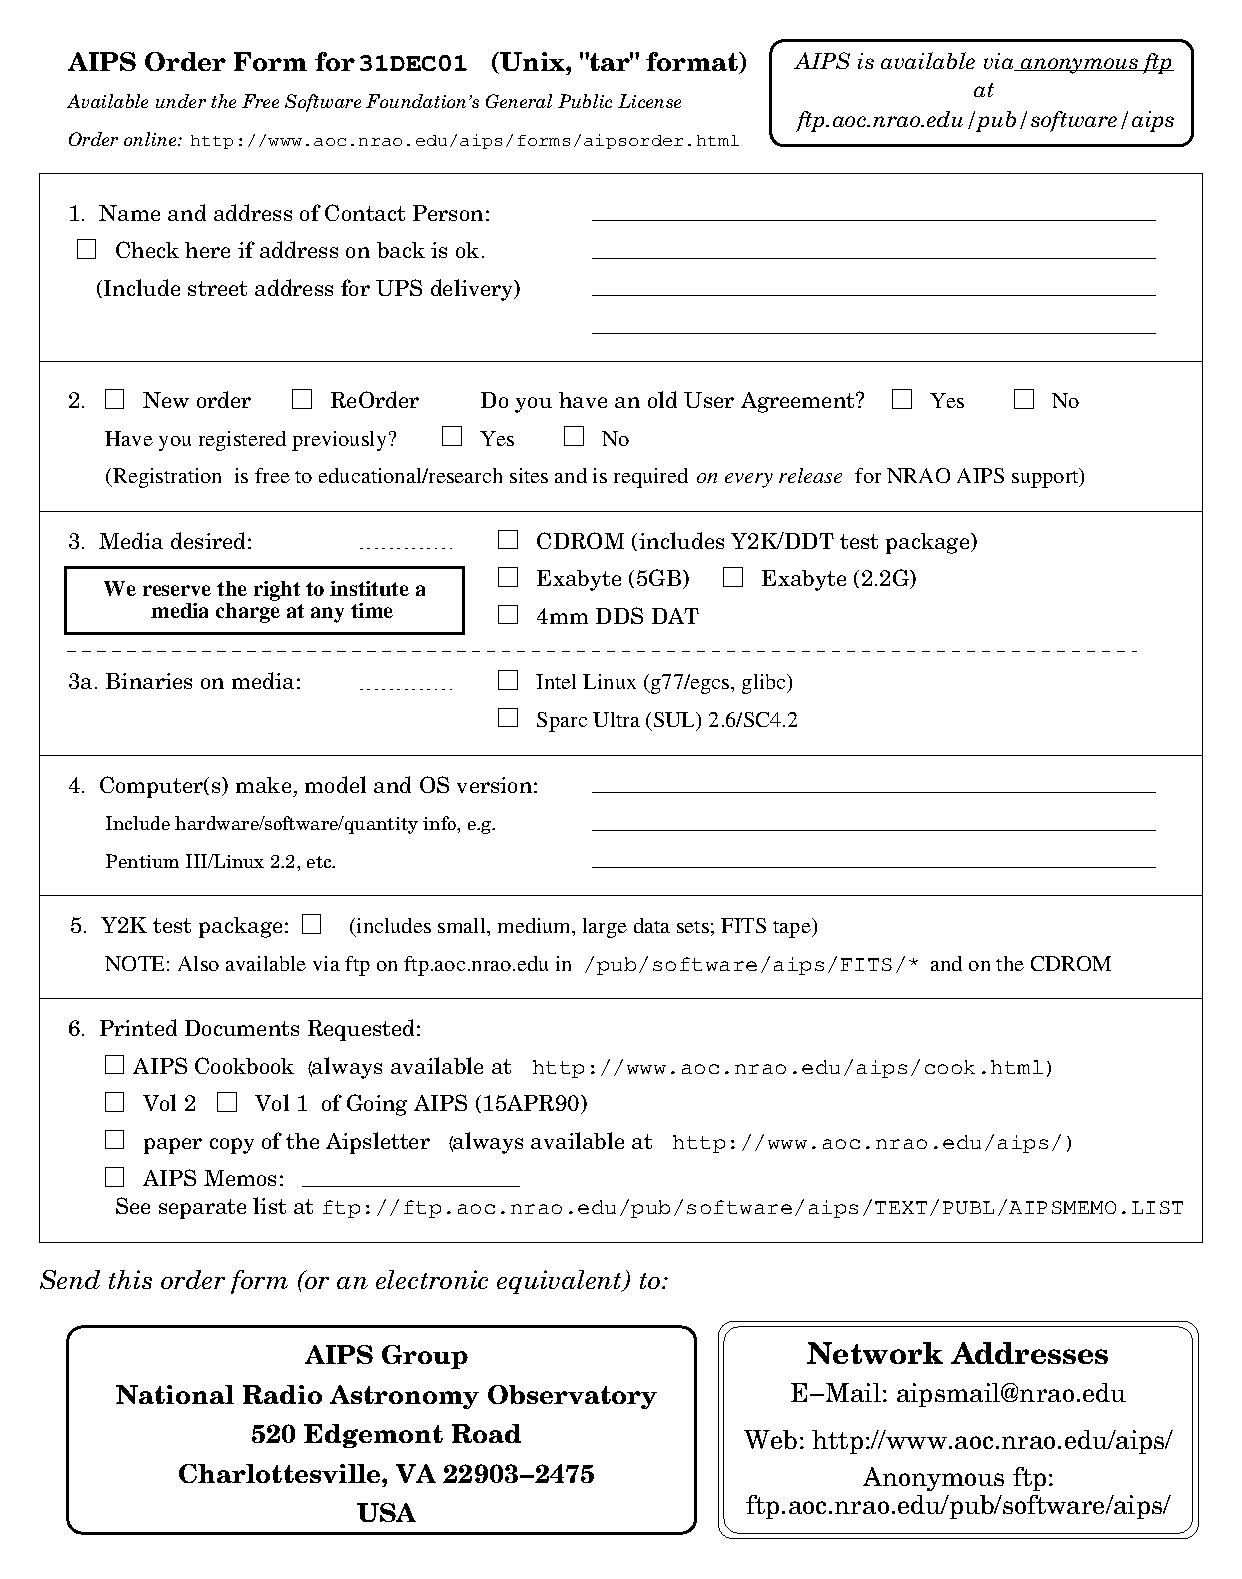
\includegraphics{FIG/AIPSORDER.PS}}}
%\vfill\eject
\vbox to 4.4in{
\vspace{12pt}
%\centerline{\rotatebox{-90}{\resizebox{!}{3.5in}{%
%\includegraphics{FIG/Mandrill.color.plt}}}}
\centerline{\resizebox{!}{3.5in}{\includegraphics{FIG/Mandrill.eps}}}
\vspace{12pt}
\centerline{{\huge \tt \AIPRELEASE}}
\vspace{12pt}
\vfill}
\phantom{...}
\centerline{\resizebox{!}{!}{\includegraphics{FIG/AIPSLETS.PS}}}

\end{document}
